\documentclass[11pt,a4wide]{article}
\usepackage{verbatim}
\usepackage{listings}
\usepackage{graphicx}
\usepackage{a4wide}
\usepackage{color}
\usepackage{amsmath}
\usepackage{amssymb}
\usepackage[dvips]{epsfig}
\usepackage[T1]{fontenc}
\usepackage{cite} % [2,3,4] --> [2--4]
\usepackage{shadow}
\usepackage{hyperref}
\usepackage[squaren]{SIunits}

\setcounter{tocdepth}{2}
\usepackage{url} %url + line break

\renewcommand{\vec}{\mathbf}
\newcommand{\dm}[1]{\mathrm{d}#1}
\newcommand{\ihat}{\hat{\textbf{\i}}}
\newcommand{\jhat}{\hat{\textbf{\j}}}
\newcommand{\khat}{\hat{\textbf{k}}}
\providecommand{\e}[1]{\ensuremath{\times 10^{#1}}}


\lstset{language=c++}
\lstset{alsolanguage=[90]Fortran}
\lstset{basicstyle=\small}
\lstset{backgroundcolor=\color{white}}
\lstset{frame=single}
\lstset{stringstyle=\ttfamily}
\lstset{keywordstyle=\color{red}\bfseries}
\lstset{commentstyle=\itshape\color{blue}}
\lstset{showspaces=false}
\lstset{showstringspaces=false}
\lstset{showtabs=false}
\lstset{breaklines}


%lager heftig forside:
\newcommand*{\titleAT}{\begingroup % Create the command for including the title page in the document
\newlength{\drop} % Command for generating a specific amount of whitespace
\drop=0.1\textheight % Define the command as 10% of the total text height

\rule{\textwidth}{1pt}\par % Thick horizontal line
\vspace{2pt}\vspace{-\baselineskip} % Whitespace between lines
\rule{\textwidth}{0.4pt}\par % Thin horizontal line

\vspace{0.5\drop} % Whitespace between the top lines and title
\centering % Center all text
\textcolor{black}{ % Red font color
{\Huge Atomic modeling of argon}\\[0.75\baselineskip] % Title line 1
%{\Large Tema:}\\[0.75\baselineskip] % Title line 2
%{\Huge Lydmåling og hørselstesting} % Title line 3
} 

\vspace{0.25\drop} % Whitespace between the title and short horizontal line
\rule{0.3\textwidth}{0.4pt}\par % Short horizontal line under the title
\vspace{0.25\drop} % Whitespace between the thin horizontal line and the author name

{\Large \textsc{Project 5, FYS-3150\\[0.75\baselineskip] \normalsize{Ina K. B. Kullmann, candidate nr: 20}
}}\par % Author name

%\vfill % Whitespace between the author name and publisher text

\vspace{0.25\drop} % Whitespace between the title and short horizontal line
\rule{0.3\textwidth}{0.4pt}\par % Short horizontal line under the title
\vspace{0.25\drop} % Whitespace between the thin horizontal line and the author name

\begin{abstract}
The aim of this project is to numerically find the critical temperature for the two dimentional Ising model by using the metropolis algorithm. We will first test the implementation of the algorithm carefully, first by comparing with theoretical values calculated for a small system. Then we will see if the algorithm behaves as expected according to our physical intuition for a larger system.

When we have found a estimate for the critical temperature we will compare it to Lars Onsagers analytical result.

\end{abstract}
\vspace*{0.25\drop} % Whitespace under the publisher text

\begin{center}
{ \scriptsize \noindent All source codes can be found at: \url{https://github.com/inakbk/molecular-dynamics-fys3150}. }
\end{center}

\rule{\textwidth}{0.4pt}\par % Thin horizontal line
\vspace{2pt}\vspace{-\baselineskip} % Whitespace between lines
\rule{\textwidth}{1pt}\par % Thick horizontal line

\endgroup}
%kode slutt for heftig forside


\begin{document}
%\maketitle
\titleAT % This command includes the title page


\newpage
\tableofcontents
\newpage

\section{Introduction}

Molecular dynamics (MD) is a computer simulation method used to study atoms and molecule structure and movement. In a MD simulation the atoms or molecules are allowed to interact trough a force given by a potential for a given time. This makes it possible to study the systems development over time. 

MD is a a type of N-body simulation since the simulation often consists of a large number of atoms or molecules. It is therefore possible to use MD to study stastistical properties of a large system consisting of N such atoms or molecules. For systems that obey the ergodic hypothesis the evolution of a single molecular dynamics simulation may be used to determine macroscopic thermodynamic properties of the system. This is because the time averages of an ergodic system correspond to microcanonical ensemble averages\footnote{\url{https://en.wikipedia.org/wiki/Molecular\_dynamics} 3.dec 11:25}.

Often the main motivation to use Molecular dynamics is that it is not possible to determine properties of the system analytically because of the large number of particles. The main limitation for the numerical simulation is the computer recources available, but also cumulative errors in the numerical integration. The first is solved by applying periodic boundary conditions while the latter is solved by proper selection of algorithms and parameters. In this paper we will have a look at two numerical integration methods; the Euler-Cromer method and the Velocity Verlet integrator. 


In this paper we will study the properties of a large system consisting of Argon atoms. And compare with experimental data(?). We will have a constant number of particles, a constant volume and a more or less constant engergy (depending on the integrator). We are more interested in the statistical properties of the system than in the individual motion of each of the particles. We want to sample microstates from the microcanonical ensemble (NVE).
(?se over avsnittet over?)


The applications of MD is many ranging from chemical physics, materials science and the modelling of biomolecules.
What areas of physics can it be used in? Chemistry and biology?(fra oppg)
see 'Areas of application and limitations' at \url{https://en.wikipedia.org/wiki/Molecular\_dynamics} and google




\section{Theory}


\section{Numerical methods}


\subsection{Creating the lattice}
We want to start out the simulation with the atoms in a crystal structure. We will choose the face-centered cubic (FCC) lattice which is a stable structure for the Lennard-Jones potential that will be used. The lattice is build up by unit cells, a group of attoms, so that a larger system can be created by repeating these cells in space. The FFC lattice unit cell is of size $b \angstrom $ and consists of four atoms with local coordinates
\begin{align}
	\vec r_1 &= 0 \ihat + 0 \jhat + 0 \khat,\\
	\vec r_2 &= \frac{b}{2} \ihat + \frac{b}{2} \jhat + 0 \khat,\\
	\vec r_3 &= 0 \ihat + \frac{b}{2} \jhat + \frac{b}{2} \khat,\\
	\vec r_4 &= \frac{b}{2} \ihat + 0 \jhat + \frac{b}{2} \khat.
\end{align}
where $b=5.26$ is the lattice constant. We want to construct a larger system with $N\times N\times N$ such unit cells next to each other. The orgin of unit cell $(i,j,k)$ is
\begin{align}
	\vec R_{i,j,k} = i \hat{\textbf{u}}_1 + j \hat{\textbf{u}}_2 + k \hat{\textbf{u}}_3,
\end{align}
where $i=0,1,..., N_x-1, j=0,1,..., N_y-1, k=0,1,..., N_z-1$. The unit vectors of the unit cells are scaled with the lattice constant $b$ so that
\begin{align}
	\hat{\textbf{u}}_1 = b\ihat, \quad \hat{\textbf{u}}_2 = b\jhat, \quad \hat{\textbf{u}}_3 = b\khat.
\end{align}

The coordinates of particle one to four is then given by:

\begin{minipage}{0.2\textwidth}
\begin{align*}
x_1 &= 0 + ib\\
y_1 &= 0 + jb \\
z_1 &= 0 + kb
\end{align*}
\smallskip
\end{minipage}
\begin{minipage}{0.25\textwidth}
\begin{align*}
x_2 &= \frac{1}{2} + ib\\
y_2 &= \frac{1}{2} + jb \\
z_2 &= 0 + kb
\end{align*}
\smallskip
\end{minipage}
\begin{minipage}{0.25\textwidth}
\begin{align*}
x_3 &= 0 + ib\\
y_3 &= \frac{1}{2} + jb \\
z_3 &= \frac{1}{2} + kb
\end{align*}
\smallskip
\end{minipage}
\begin{minipage}{0.25\textwidth}
\begin{align*}
x_4 &= \frac{1}{2} + ib\\
y_4 &= 0 + jb \\
z_4 &= \frac{1}{2} + kb
\end{align*}
\smallskip
\end{minipage}

Each of the sides of the simulation box has the length $L = bN$ so that the size of the whole system or the volume of the cubic lattice is given by $V = L^3 = (bN)^3$. The density of the system is then:
\[
\rho = \frac{M_{tot}}{V} = \frac{4*N^3*m}{(bN)^3} = \frac{4m}{b^3}
\]
where $m$ is the mass of one atom and is equal for all the atoms. We can see that the density will be constant as long as the mass and the lattice constant is held constant. 

should include particle density not mass density! (?)


\subsection{The Maxwell-Boltzmann distrubution (giving velocities)}
The atoms are usually given velocities according to the Maxwell-Boltzmann distribution so that
\begin{align}
	\label{eq:maxwell_boltzmann}
	P(v_i)\dm{v_i} = \left(\frac{m}{2\pi k_B T}\right)^{1/2} \exp\left(-\frac{m v_i^2}{2k_B T}\right) \dm{v_i},
\end{align}
where $m$ is the mass of the atom, $k_B$ is Boltzmann's constant and $T$ is the temperature. We recognize this as a normal distribution with zero mean and standard deviation $\sigma = \sqrt{k_B T/m}$. This is a good choice because bla bla bla bla (?) 


But this will result in a nonzero net momentum in the system which we will remove. The momentum in a given direction for one atom is $p_{i} = mv_i$ where the mass is $m$ and $v_i$ is the velocity in direction $i$. The total momentum in one direction, assuming that all particles have the same mass, is given by:
\[
p_{tot} = m(v_{i,1} + v_{i,2} + v_{i,3} + \dots + v_{i,n})
\]
where $n$ is the total number of atoms in the simulation. 

We want to remove this momentum evenly from all the particles. The momentum we want to remove from each particle is then:
\[
p_{rm} = \frac{p_{tot}}{n}
\]
so that $p_i'$ is the momentum for one particle after removing the total momentum:
\[
p_i' = p_i - p_{rm} 
\]
If we write this out
\begin{align*}
mv_i' &= mv_i - \frac{m(v_{i,1} + v_{i,2} + v_{i,3} + \dots + v_{i,n})}{n} \\
\Rightarrow v_i' &= v_i - \frac{v_{i,1} + v_{i,2} + v_{i,3} + \dots + v_{i,n}}{n} \\
&= v_i - \overline{v_i}
\end{align*}
We see that to remove the total momentum we only have to substract the average velocity from each of the particles velocity. 

\subsection{Periodic boundaryconditions (PBCs)} 
To avoid problems with boundary effects we will apply periodic boundary conditions. This has a great analogy to 'old' video games such as Snake 2. If the snake head passes through one side of box, it re-appears on the opposite side with the same velocity. In the system of atoms this would mean that if an atom should leave the simulation box at one side it will enter on the oposite side with the same values for the physical parameters as it had before it left. This also implies that an attom at the edge of the box will interact with an atom at the opposite side of the box so that every atom have the same number of 'neighbours'. 

MD simulations that use periodic boundary conditions have a large number of unit cells (defined above?), a group of atoms, so that a larger system can be created by repeating these cells in space. 

The size of the simulation box must also be large enough to prevent unphysical behaviour. If the box is too small one unit cell (a few atoms) might interact with itself. In the Snake analogy this would mean that the "head" interacts with or bites its own "tail" trough the wall which is allowed in the game, but not very physical. Thus the box size have to be large enough relative to the size of a unit cell, length of the simulation and the desired accuracy\footnote{\url{https://en.wikipedia.org/wiki/Periodic\_boundary\_conditions\#Practical\_implementation:\_continuity\_and\_the\_minimum\_image\_convention}}.


\subsection{Intergration methods} \label{sec: int_methods}
During the first implementation of the MD code we have used the Euler-Cromer method to find the next time step for the atoms. (bla bla legge til likninger?)

In MD the Velocity Verlet integrator is usually used. This is because other integration algorithms tend to drift the energy over time, which we want to avoid. The Velocity Verlet algorithm consists of three steps (in addition to computing the forces, see section \ref{sec: L-Jpot_forces})
\begin{align}
	\vec v(t + \Delta t/2) &= \vec v(t) + \frac{\vec F(t)}{m}\frac{\Delta t}{2}\\
	\vec r(t + \Delta t) &= \vec r(t) + \vec v(t + \Delta t/2)\Delta t\\
	\vec v(t + \Delta t) &= \vec v(t + \Delta t/2) + \frac{\vec F(t + \Delta t)}{m}\frac{\Delta t}{2}.
\end{align}

sympletic integrator bla bla bla?

To measure the drift of the energy we will use the standard deviation of the total energy $E$:
\[
\sigma_E = \sqrt{\langle E^2 \rangle - \langle E \rangle^2}
\]
that we will calculate using the Euler-Cromer method and the Velocity-Verlet integrator and compare the results.

Will also compare cumputing time (plot this!?)

say something more about energy drift?

(discussed in the lecture notes.?)
  see \url{https://en.wikipedia.org/wiki/Verlet\_integration\#Velocity\_Verlet} on conserved quantities
  
bla bla bla  

\subsection{The Lennard-Jones potential (interaction/forces)} \label{sec: L-Jpot_forces}

In this project we will use the Lennard-Jones potential which is a mathematically simple model that approximates the interaction between a pair of neutral atoms or molecules. Due to its computational simplicity, the Lennard-Jones potential is used extensively in computer simulations even though more accurate potentials exist\footnote{\url{http://en.wikipedia.org/wiki/Lennard-Jones_potential}}.

The potential calculates the energy between two atoms $i$ and $j$ as
\begin{align}
	U(r_{ij}) = 4\epsilon\left[\left(\frac{\sigma}{r_{ij}}\right)^{12} - \left(\frac{\sigma}{r_{ij}}\right)^6\right],
\end{align}
where $r_{ij} = |\vec r_i - \vec r_j|$ is the distance from atom $i$ to atom $j$, $\epsilon$ is the depth of the potential well (units energy) and $\sigma$ is the distance at which the potential is zero. 

The parameters in the potential can be fitted to reproduce experimental data. For argon, optimal values of the parameters are:
\begin{align}
	\frac{\epsilon}{k_B} = \unit{119.8}{\kelvin}, \sigma=\unit{3.405}{\angstrom}.
\end{align}
With these parameters the L-J potential reproduces equilibrium thermodynamic properties that are in good agreement with experimental values for argon.

In our code, we use the so called MD units (see appendix \ref{sec:units}). (finne enheten og verdier til parameterne?)

%The equation of state for this system is the van der Waals equation of state. Phases such as solid, liquid and gas are reproduced from this simple model with phase transitions and everything which is remarkable.(?)

The force is calculated by taking the negative gradient of the potential
\begin{align}
	\vec F(r_{ij}) = -\nabla U(r_{ij}),
\end{align}
giving the $x$-component (the other components are calculated the same way)
\begin{align}
	F_x(r_{ij}) = -\frac{\partial U}{\partial r_{ij}}\frac{\partial r_{ij}}{\partial x_{ij}},
\end{align}
where $x_{ij}$ is the $x$-component of $\vec r_{ij}$. Calculating the differensials separately:
\begin{align*}
\frac{\partial U}{\partial r_{ij}} &= \frac{\partial }{\partial r_{ij}} 4\epsilon\Big[\Big(\frac{\sigma}{r_{ij}}\Big)^{12} - \Big(\frac{\sigma}{r_{ij}}\Big)^6 \Big] =  4\epsilon\Big[ \sigma^{12}\frac{\partial }{\partial r_{ij}} r_{ij}^{-12} - \sigma^6 \frac{\partial }{\partial r_{ij}}r_{ij}^{-6} \Big] \\
&= 4\epsilon\Big[ -12\sigma^{12} r_{ij}^{-13} -(-6) \sigma^6 r_{ij}^{-7} \Big] = \frac{24\epsilon}{\sigma} \Big[\Big(\frac{\sigma}{r_{ij}}\Big)^{7} - 2\Big(\frac{\sigma}{r_{ij}}\Big)^{13} \Big] \\
r_{ij} &= |\vec{r_i} - \vec{r_j} | = | x_i\ihat + y_i\jhat + z_i\khat - x_j\ihat + y_j\jhat + z_j\khat | = | (x_i - x_j)\ihat + (y_i - y_j)\jhat + (z_i - z_j)\khat | \\
&= \sqrt{(x_i - x_j)^2 + (y_i - y_j)^2 + (z_i - z_j)^2} = \sqrt{x_{ij}^2 + y_{ij}^2 + z_{ij}^2} \\
\frac{\partial r_{ij}}{\partial x_{ij}} &= \frac{\partial}{\partial x_{ij}} \sqrt{x_{ij}^2 + y_{ij}^2 + z_{ij}^2} = \frac{1}{2r_{ij}}\cdot 2x_{ij} = \frac{x_{ij}}{r_{ij}}
\end{align*}
gives
\begin{align*}
F_x(r_{ij}) &= -\frac{24\epsilon}{\sigma} \Big[\Big(\frac{\sigma}{r_{ij}}\Big)^{7} - 2\Big(\frac{\sigma}{r_{ij}}\Big)^{13} \Big]\cdot \frac{x_{ij}}{r_{ij}} \\
&= \frac{24\epsilon}{\sigma^2} \Big[2\Big(\frac{\sigma}{r_{ij}}\Big)^{14} - \Big(\frac{\sigma}{r_{ij}}\Big)^{8} \Big]x_{ij}
\end{align*}
The force in y and z direction can be calculated the same way giving:
\begin{align*}
\vec F &= F_x\ihat + F_y \jhat + F_z\khat \\
&= \frac{24\epsilon}{\sigma^2} \Big[2\Big(\frac{\sigma}{r_{ij}}\Big)^{14} - \Big(\frac{\sigma}{r_{ij}}\Big)^{8} \Big]\Big(x_{ij}\ihat + y_{ij}\jhat + z_{ij}\khat \Big)
\end{align*}



(another section???)

In section \ref{sec: int_methods} we see that to calculate the next time step for the particles we need to calculate the forces. This is very time consuming because we have to sum over all pairs of particles to find the force for one particle. Therefore a lot of time can be saved if the code for the calculation of forces is as efficient as possible.

A better numerical expression for the force is
\begin{align*}
\vec F(r_{ij}) &= \frac{24\epsilon}{\sigma^2} \Big(\frac{\sigma}{r_{ij}}\Big)^2\Big(\frac{\sigma}{r_{ij}}\Big)^6\Big[2\Big(\frac{\sigma}{r_{ij}}\Big)^{6} - 1 \Big]\Big(x_{ij}\ihat + y_{ij}\jhat + z_{ij}\khat \Big)\\
&= 24\epsilon\sigma^6r_{ij}^{-2}r_{ij}^{-6}\big(2\sigma^6r_{ij}^{-6} - 1\big)
\end{align*}
and for the potential energy
\begin{align*}
U(r_{ij}) = 4\epsilon\sigma^6r_{ij}^{-6}\big(\sigma^6r_{ij}^{-6} - 1\big)
\end{align*}
so that the powers of $r_{ij}$ is calculated as few times as possible, $r_{ij}^{-6}$ can be calculated just once for each loop (define?).  

Another smart way to make a more efficient code when calculating the forces is to realize that in the limit $r_{ij}\rightarrow \infty$ both the force and the potential energy is zero. In figure \ref{fig: force_potential} the potential energy (red) and the force (blue) plotted against the distance between two atoms $r_{ij}$. We can see that the energy and the force reaches zero for large values of $r_{ij}$.  The point for which the potential energy and the force is nearly zero, $r_{cut}$, is marked with a dot in the figure. A good approximation is therefore to stop calculating forces and energies for distances larger than $r_{cut}$ and set all forces and energies for $r_{ij} > r_{cut}$ to zero.

\begin{figure}
\centering
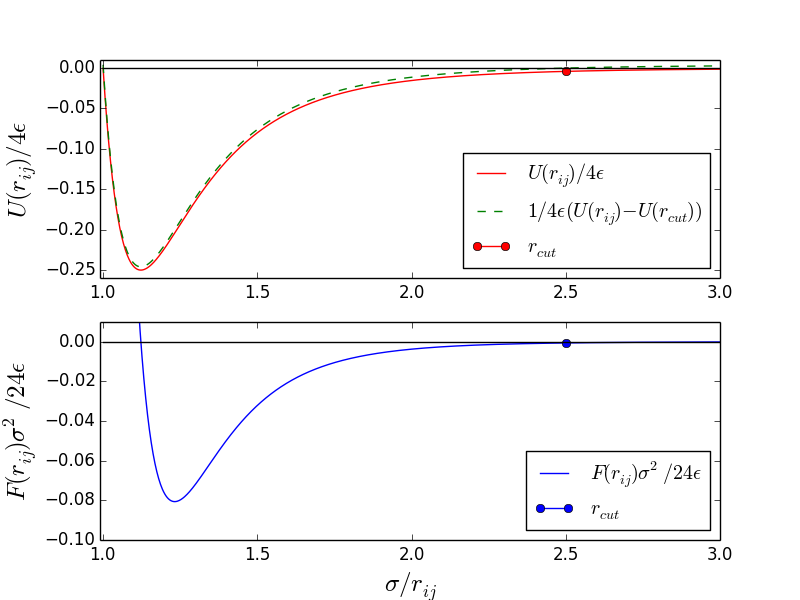
\includegraphics[width = 0.8\textwidth]{plots_theory/force_potential.png}
\caption{\textbf{Top:} The Lennard-Jones potential (red), or the potential energy $U(r_{ij})$ between two atoms $i$ and $j$ plotted against the distance between atom $i$ and $j$, $r_{ij}$. The point $(r_{cut},U(r_{cut}))$ is marked with a  red dot. The shifted potential function is also plotted in green. \textbf{Bottom:}  The force (blue) between two atoms $i$ and $j$ plotted against the distance between atom $i$ and $j$, $r_{ij}$. The point $(r_{cut}, F(r_{cut}))$ is marked with a blue dot.}
\label{fig: force_potential}
\end{figure}

The implementation of $r_{cut}$ will save the algorithm a lot of time and still be a good approximation since the force and the potential energy is esensially zero anyway. The only problem is that the potential energy function will be discontinuously at the point $r_{cut}$ when the energy is set to zero after $r_{cut}$. A solution to this is to shift the potential function slightly so that the energy is zero at $r_{cut}$ and still set to zero for $r_{ij}>r_{cut}$. The shifted potential function is marked with green in figure \ref{fig: force_potential}. This will only shift the values for the potential and total energy, but it will not affect the physics of the problem. The statistical properties of the system will not be affected by the shift in energy. 


\paragraph{The minimum image convention} (due to calculation of forces)
When an atom leave the simulation box it must re-enter the box on the opposite side. An atom at the edge of the simulation box must also interact with an atom at the other side of the box 'through' the wall, or interact with the image of the simulation box. But this atom is also contained inside the box so the atoms interact twice, once through the wall and once from across the box. To avoid counting this interaction twice we will apply the minimum image convention. An atom will interact with the other atoms only once and then choose the image (or the simulation box) that gives the minimum distance\footnote{\url{https://en.wikipedia.org/wiki/Periodic\_boundary\_conditions\#Practical\_implementation:\_continuity\_and\_the\_minimum\_image\_convention}}:
%This is because we want to avoid extensive mathematical calculations of pairwise interactions with all particle inside or outside the box. MIC is a way of providing a cutoff distance over which we are not calculating pairwise potential. The cutoff is usually half the box length. This means if distance between particle i and particle j is more than L/2, you will neglect the pairwise potential between i & j, instead you will consider potential between i & neareset image of j, hence the term Minimum Image.

\begin{lstlisting}
if(periodic_x) then
  dx = x(j) - x(i)
  if (dx >   x_size * 0.5) dx = dx - x_size
  if (dx <= -x_size * 0.5) dx = dx + x_size
endif
\end{lstlisting}

(include drawing??)

This leads to two possible strategic choices: (A) 'fold back' particles into the simulation box when they leave it, or (B) let them go on into the other side of the box?

....ahh, this is relevant for computing forces/potentials!
An atom which has passed through one face of the simulation box should re-enter through the opposite face-or its image should do it. Evidently, a strategic decision must be made: Do we (A) “fold back” particles into the simulation box when they leave it, or do we (B) let them go on (but compute interactions with the nearest images)? The decision has no effect on the course of the simulation, but if the user in interested in mean displacements, diffusion lenghts, etc., the second option is preferable.




  
  
\subsection{Calculating physical properties of the system}
The total potential energy $V$ in the system is computed by summing over all pairs of atoms (counting each pair only once) 
\begin{align}
	V = \sum_{i>j} U(r_{ij}).
\end{align}
where $U(r_{ij})$ are the Lennard-Jones potential given in section \ref{sec: L-Jpot_forces}. The kinetic energy is defined as
\begin{align}
	E_k = \sum_{i=1}^{N_\text{atoms}} \frac{1}{2} m_i v_i^2,
\end{align}
where $m_i$ and $v_i$ is the mass and the speed of atom $i$. The total energy of the system is then $E = V + E_k$. (which we will study if is conserved or not, see $\sigma_E$ ??)

We will also calculate an estimate of the temperature through the equipartition theorem\footnote{See for example D. Schroeder's \textit{An Introduction to Thermal Physics} for details. better reference?}
\begin{align}
	\langle E_k \rangle = \frac{3}{2}N_\text{atoms} k_B T.
\end{align}
We can use this to define an \textit{instantaneous} temperature
\begin{align}
	\label{eq:temperature}
	T = \frac{2}{3}\frac{E_k}{N_\text{atoms} k_B}.
\end{align}


\paragraph{The diffusion constant} of the system can be used to measure the melting temperature. We use the Einstein relation that relates the so called mean square displacement (MSD) to the diffusion constant
\begin{align}
	\langle r^2(t) \rangle = 6Dt,
\end{align}
where $D$ is the diffusion constant, $t$ is time. The mean square displacement for atom $i$ is calculated as
\begin{align}
	r_i^2(t) = |\vec r_i(t) - \vec r_i(0)|^2,
\end{align}
where $\vec r_i(t)$ is the position of atom $i$ at time $t$. 

The diffusion constant is then given by
\begin{align*}
D = \frac{\langle r^2(t) \rangle}{6t} = 
\end{align*}
(for a given temperature ($T_i$ ?).)

Atoms in a solid will not diffuse (move?) much, so a solid will have a diffusion constant close to zero. A plot of the diffusion constant as a function of temperature will therefore reveale the melting temperature because the solid melts when the diffusion constant is non zero.


\centering
\rule{0.3\textwidth}{0.4pt}\par % Short horizontal line under the title  

\end{document}







